\documentclass[11pt]{article}
\usepackage[margin=1in]{geometry}
\usepackage[T1]{fontenc}
\usepackage{amsmath,amssymb,booktabs,graphicx,hyperref,xcolor,array,caption}
\usepackage[numbers,sort&compress]{natbib}
\newcommand{\todo}[1]{{\color{red}[\textbf{TODO:} #1]}}
\newcommand{\cn}[1]{{\color{orange}[\textbf{CITATION NEEDED:} #1]}}
\newcommand{\verify}[1]{{\color{blue}[\textbf{VERIFY:} #1]}}

\title{Measuring the Simulation Gap in Root Cause Analysis for CNC Milling:\\
A Physics-Based Simulator Grounded in Real Multi-Sensor Data}
\author{\textit{Author names and affiliations to be added}}
\date{\textbf{DRAFT} --- target venue not yet chosen; several results are incomplete (see Section~\ref{sec:limits})}

\begin{document}
\maketitle

\begin{abstract}
Root cause analysis (RCA) of machining faults lacks public data with ground-truth causes, so RCA methods are routinely evaluated on simulators whose generator is also used to build the diagnostic nodes.
We build a regenerative-milling simulator (delay-differential equations with helical flutes and edge forces) and ground its healthy baseline in a real multi-sensor milling dataset by modelling accelerometer and microphone spectra and their dependence on cutting conditions.
Fault effects (stiffness, damping, tool wear, depth, spindle speed) are injected through the simulator and scaled by an effect-size calibration against real anomalous cuts.
We then evaluate six causal RCA algorithms on a 14-node graph following a root-cause-ranking protocol.
When diagnostic nodes and test faults come from the same generator, top-1 accuracy at $m{=}10$ interventional samples is 0.52--0.98 (0.80--0.98 for five of six algorithms); when the simulator's physical parameters are shifted at test time it falls to 0.35--0.71, and the ordering of methods changes.
Ablations show that this accuracy comes from supervised estimates of the root-cause nodes, not from the causal graph: replacing the graph by a shuffled or an empty one leaves every algorithm unchanged, and label-free nodes drop accuracy to near chance.
The simulated healthy baseline is still distinguishable from real data (classifier two-sample test, balanced accuracy $0.82\pm0.04$), and a comparison with a real defective tool shows large shifts at low frequencies and in non-synchronous indices that none of the simulated faults reproduces.
We therefore present the results as a measurement of how strongly simulated RCA benchmarks depend on generator assumptions and node construction, not as evidence of real-world diagnostic accuracy.
\end{abstract}

\section{Introduction}
Diagnosing why a milling operation misbehaves (loose fixture, worn tool, excessive depth, unsuitable spindle speed) requires knowing which physical cause produced the sensor signals.
Real datasets rarely record causes; they record sensor streams and, at best, expert labels of ``normal'' or ``abnormal''.
The recently released MSM dataset \citep{kim2026msm} is a rare multi-sensor milling collection with expert labels, but it does not provide root-cause annotations for most anomalies.
Causal RCA methods, several developed for microservices \citep{ikram2022rcd,pham2024baro} and related outlier-explanation settings \citep{orchard2025}, take an observational dataset of healthy behaviour and a few anomalous samples, and rank graph nodes by how much their mechanism changed.
Applying them to machining needs a source of faulty data with known causes, and the natural source is a simulator.

\paragraph{The problem.}
A simulator-based RCA benchmark is only informative if the simulated data resemble real data and if the diagnostic procedure does not exploit the simulator itself.
Both conditions are hard to check: real root causes are unavailable, and nodes of the causal graph are usually derived from, or trained on, the same generator that produces the test faults.

\paragraph{What we do.}
(1) We implement a regenerative-milling simulator for the tool used in MSM, with every parameter tagged as fixed from a catalogue, learned from data, or assumed (Appendix~\ref{app:registry}).
(2) We build the healthy baseline from real spectra rather than from the simulator, and report honestly how close it is (classifier two-sample test).
(3) We inject simulated faults and calibrate their scale by effect size on real anomalous cuts.
(4) We run six causal RCA algorithms and test them with and without a mismatch between the generator used to build the nodes and the one used to generate the faults.

\paragraph{Main findings.}
(i) Top-1 accuracy at $m{=}10$ drops from $0.80$--$0.98$ (five of six algorithms) to $0.35$--$0.71$ (all six) under moderate shifts of the simulator's stiffness, damping and force coefficients, and the ranking of the algorithms changes.
(ii) The causal graph is irrelevant in this benchmark: shuffled and empty graphs give the same accuracy as the physical graph, and nodes built without simulator labels give near-chance accuracy, so the benchmark measures the quality of supervised node estimators rather than causal reasoning.
(iii) A real defective tool shifts low-frequency energy and non-synchronous indices by several standard deviations, and none of the simulated faults reproduces this.

\paragraph{What we do not show.}
We have no validation of the RCA ranking on real root causes (the real defective-tool data test only the signature of one cause, on a different tool than the one simulated), and the simulated healthy baseline is distinguishable from real data (Section~\ref{sec:limits}).

\section{Related Work}
\paragraph{Regenerative chatter and milling simulation.}
Regenerative chatter stability and its analytical and time-domain treatment are surveyed by \citet{altintas2020}; we use the zero-order stability-lobe approximation and a time-domain delay model in that tradition.

\paragraph{Machining datasets.}
\citet{kim2026msm} release synchronised accelerometer, microphone, current and controller data from three machines with expert anomaly labels (normal, abnormal, defective tool). We use a subset (Section~\ref{sec:data}).

\paragraph{Causal root cause analysis.}
RCD \citep{ikram2022rcd} localises root causes with conditional-independence tests, BARO \citep{pham2024baro} uses multivariate Bayesian online change-point detection, and \citet{orchard2025} study root causes of outliers without full structural knowledge; our ``Smooth Traversal'' baseline follows the repository's description attributed to this work \verify{confirm that the implemented algorithm matches the paper}.
BRCD, RCG and SimpleRCA are implemented in our codebase from the repository's descriptions \cn{BRCD (Lee, Zhou, Kocaoglu, ICML 2026), RCG (UAI 2025), SimpleRCA (Fang 2025): the author confirms the sources; bibliographic entries still to be added}.

\paragraph{Calibrating simulators to data.}
Calibration of computer models with a model-discrepancy term is classical \citep{kennedy2001}; domain randomisation \citep{tobin2017}, adversarial refinement of simulated data \citep{shrivastava2017} and simulation-based inference \citep{cranmer2020} are alternatives. We considered adversarial refinement but did not use it because of the small number of real cuts; we use a classifier two-sample test only as a diagnostic \cn{Lopez-Paz and Oquab 2017; Gretton et al. 2012}.

\section{Data}\label{sec:data}
We use datasets 5 and 6 of machine \texttt{imi\_vm20i} (Hurco, wet cutting, AA~6061): tool 2SE0250IX150A (2 flutes, 6.35~mm, flute length 38.1~mm, per the manufacturer catalogue), axial depth 38.1~mm, spindle speed 9000--12000~rpm, radial depth $a_e\in\{0.0635,0.1905,0.3175\}$~mm, up and down milling.
This gives 73 cuts (48 labelled normal, 25 abnormal); each cut is split into three 0.3~s windows (219 windows).
We verified that the spindle speed and feed in the label files equal the controller-recorded values (ratio 1.000).
In these two datasets the abnormal label is strongly associated with up-milling rather than with a specific root cause (all 36 down-milling cuts are normal).
Cuts with a documented root cause (defective tools, clamp failure, excessive depth) exist in other datasets but use different tools, and we could not complete their analysis (Section~\ref{sec:limits}).

\section{Method}
\subsection{Simulator}
The tool-tip displacement follows modal dynamics driven by cutting forces; the chip thickness of each flute slice depends on the current and delayed displacement.
For each of the $N_z{=}8$ axial slices of a flute, with helix lag $\psi(z)=2z\tan\beta/D$, the elemental forces are
\begin{equation}
dF_t=(K_t h+K_{te})\,dz,\qquad dF_r=(K_r K_t h+K_{re})\,dz,
\end{equation}
where $h$ is the chip thickness (clipped at 0 and a cap), $K_{te},K_{re}$ are edge-force coefficients and $\beta{=}30^\circ$ (manufacturer series feature list; medium confidence).
Spindle imbalance adds a synchronous rotating force $U\Omega^2$.
With helix and edge forces switched off the implementation reproduces our earlier straight-flute reference to $7\times10^{-16}$ relative error.
The zero-order stability-lobe computation reproduces the repository's previous implementation exactly on the same transfer function, and a time-domain grid agrees with the lobe prediction on 79\% of $(n,a)$ points (Figure~\ref{fig:lobes}); the disagreement is concentrated at moderate depth, where the zero-order approximation is known to be conservative for half-immersion cuts.

\begin{figure}[t]\centering
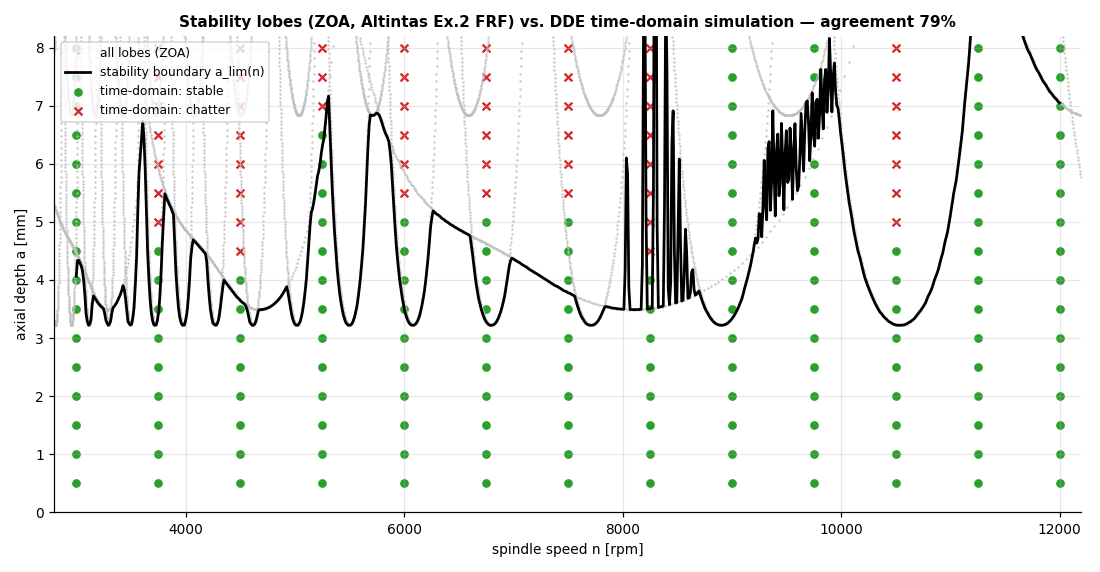
\includegraphics[width=0.78\linewidth]{figures/exp1_lobes_validation.png}
\caption{Stability lobes (zero-order approximation, 4-flute reference transfer function) and time-domain simulation outcomes on a speed--depth grid.}\label{fig:lobes}
\end{figure}

\subsection{Provenance of every parameter}
Following a fixed policy, a parameter is \emph{fixed} if a verified source gives its value for this exact tool and context, taken from a \emph{range} if a source gives one, and \emph{learned} from data otherwise; values with no source or data are marked \emph{assumed}.
Appendix~\ref{app:registry} lists each parameter, its tier and the verification status.
Cutting-force coefficients for this tool and material, the tool-tip transfer function and the spindle imbalance had no usable source in our search and are therefore not fixed; we found no verified range for them either.
In practice our direct attempts to learn them failed (Section~\ref{sec:neg}), so the simulator's physical parameters are nominal values, which is itself an assumption.

\subsection{Healthy baseline from real spectra}
For each 0.3~s window we estimate the one-sided power spectral density of the two accelerometer channels and the microphone, and summarise it by a piecewise-linear envelope over log-frequency (18 knots; knot values are band-averaged linear power so that total energy is preserved) plus the rms amplitude of the first eight harmonics of the spindle frequency $f_0=n/60$.
The parameters are regressed on the cutting conditions (kernel ridge on $\log n$, $\log a_e$, $\log f$, direction, label) and the residuals are decomposed by one-way variance analysis into a between-cut and a within-cut component on twelve principal directions, with out-of-sample residuals.
Synthetic windows are generated by shaping complex Gaussian spectra with the envelope and adding harmonics with random phases.
The real spectra differ clearly from white or pink noise: the accelerometer shows a flat floor, a brick-wall cut-off near 23~kHz and a cluster of peaks at 1.5--2.3~kHz that is about two orders of magnitude stronger in abnormal windows; the microphone shows a broad hump at 1--6~kHz (Figure~\ref{fig:psd}).

\begin{figure}[t]\centering
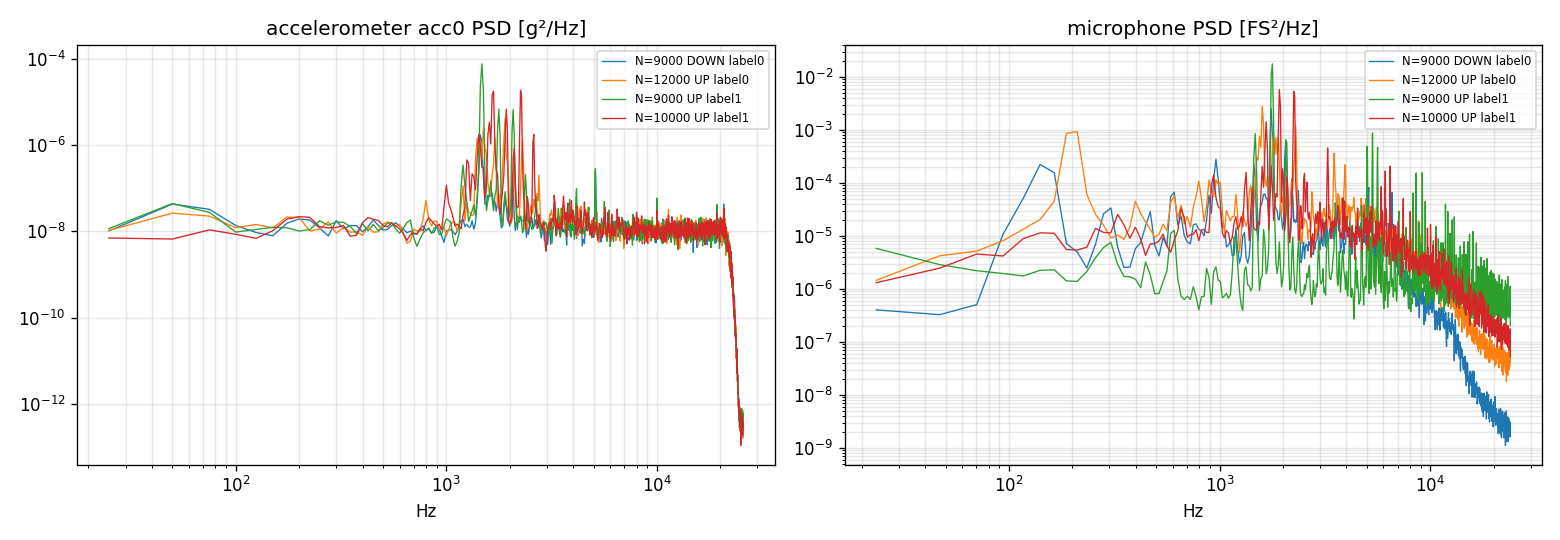
\includegraphics[width=0.95\linewidth]{figures/real_psd_examples.png}
\caption{Power spectral density of four real windows (accelerometer left, microphone right): normal and abnormal cuts at different spindle speeds.}\label{fig:psd}
\end{figure}

\subsection{Fault injection and gain calibration}
For each window and fault class we run the simulator twice at identical conditions and noise seed (healthy and faulty), and add the scaled difference $g\,(s_{\text{fault}}-s_{\text{healthy}})$ to the real-spectra baseline, with separate gains $g_{\text{acc}},g_{\text{mic}}$.
The five faults and their severity ranges (assumed, no source) are: stiffness $\times[0.4,0.9]$; damping $\times[0.3,0.8]$; tool wear $K_t\times[1.1,1.6]$ with edge forces increased; radial depth $\times[1.5,4]$; spindle speed $\pm[3\%,15\%]$.
Matching the distribution of simulated faulty features to real abnormal windows did not identify the gains (the objective was flat for small gains, Section~\ref{sec:neg}); we therefore set them by effect size, so that the mean shift of $\log_{10}$ acceleration rms and of microphone level equals the real difference between abnormal and normal windows ($+0.375$ and $+4.86$~dB), giving $g_{\text{acc}}=7.7\times10^{-6}$ and $g_{\text{mic}}=0.0116$.
Because real abnormal windows here are mainly up-milling cuts, this scale is an assumption about how strong a fault is, not an estimate of it.

\subsection{Causal RCA protocol}
We follow the root-cause-ranking protocol of the repository: a healthy dataset $D_{\mathrm{obs}}$ and $m$ anomalous samples $D_{\mathrm{int}}$ are given, and each algorithm ranks all 14 nodes; we report top-$k$ accuracy for the true root-cause node.
The nodes are five root-cause nodes (estimated stiffness, damping, tool wear, depth, and a controller-measured spindle-speed deviation) and nine sensor nodes (log acceleration, microphone level, two spectral non-synchronous indices, three accelerometer bands, two microphone bands).
The directed graph encodes physical prior knowledge (each root cause points to the sensor quantities it can affect).
The first four root-cause nodes are soft sensors: gradient-boosted regressors of the logarithm of the latent fault factor from the 30 spectral features, trained on training cuts only (out-of-fold for $D_{\mathrm{obs}}$); the spindle-speed node is the true factor plus 0.5\% reading noise.
All nodes are standardised with $D_{\mathrm{obs}}$.
Because the soft sensors are trained on labels from the same simulator, we add a \emph{shifted} test where the simulator's natural frequency, damping, stiffness, force and edge coefficients are multiplied by random factors in $[0.75,1.33]$, $[0.5,2]$, $[0.6,1.7]$, $[0.6,1.6]$ and $[0.4,2.5]$ respectively for each cut, while the soft sensors keep their nominal-parameter training.
Cuts are split by identity into 43 training and 30 test cuts, stratified by $a_e$; each test point averages 100 random draws of $m$ faulty windows per fault.

\section{Experiments}
\subsection{How realistic is the healthy baseline?}
We train the baseline model on a subset of cuts and test it on held-out cuts, using a random-forest classifier two-sample test on the four summary features and the conditions, with balanced accuracy and fold assignment by cut (0.5 means indistinguishable).
The first version of this metric used plain accuracy with five synthetic windows per real window, whose chance level is 0.83; those numbers are discarded.
Table~\ref{tab:c2st} shows the progression; the final variants remain far from 0.5 and the differences between the kernel-regression and hierarchical variants are within the spread across data splits.
Feature means match well (e.g.\ log acceleration $-1.37$ simulated vs.\ $-1.38$ real), but their dispersion and joint dependence on conditions do not.
We could not measure an empirical floor for this test because no cutting condition is repeated in the data (only three $a_e$ values and one cut per condition).
\begin{table}[t]\centering\small
\begin{tabular}{lc}
\toprule
Real-noise model variant & C2ST balanced accuracy (0.5 = indistinguishable) \\
\midrule
Linear regression, mean only & 0.986 \\
Linear regression + between/within-cut variation & 0.876 \\
Kernel ridge + stratified split, mean only (3 splits) & 0.864 $\pm$ 0.022 \\
Kernel ridge + hierarchical variation (3 splits) & 0.820 $\pm$ 0.036 \\
\bottomrule
\end{tabular}

\caption{Classifier two-sample test between real and simulated healthy windows on held-out cuts. Three-split values are mean $\pm$ standard deviation over random stratified splits. \verify{values copied from console logs; only the last run is archived}}\label{tab:c2st}
\end{table}

\subsection{A negative result: direct calibration of the delay model}\label{sec:neg}
We tried to fit the simulator's physical and sensor parameters directly to real windows with CMA-ES, matching feature distributions (MMD), later matching group means over cutting conditions.
With 15 free parameters the loss plateaued near 3 (squared errors in units of the real standard deviation) and did not converge after 35--40 generations; we stopped it by a pre-set rule.
Earlier low-MMD fits coexisted with qualitatively wrong dependence on conditions: in the real data the microphone level correlates with spindle speed at $+0.85$ while the simulation gave $0.00$, and the simulated acceleration depended on radial depth ($0.69$) where the real one did not ($0.06$).
A bug that we had to fix on the way is instructive: real features had been computed on windows of about 4~s and simulated features on 0.18~s, which inflated simulated variance threefold.
We conclude that the available data do not constrain the delay model's absolute levels, which is why we use the simulator only for fault \emph{differences}.

\subsection{Classifying simulated fault classes}
Table~\ref{tab:cls} reports six-class classification (healthy plus five faults) on 16 held-out cuts, with hyper-parameters chosen on 14 validation cuts. Tree ensembles are best; Gaussian generative models are worse, consistent with highly correlated continuous features.
These numbers hold \emph{within the simulator}.
Applying the models to real windows, 91--97\% of real normal windows are classified normal by the three tree and neighbour models, but only 51\% and 57\% by logistic regression and Naive Bayes, and 61, 64 and 72 of 75 real abnormal windows are assigned to tool wear by QDA, random forest and gradient boosting respectively.
There is no ground truth for the abnormal windows, so we read this as a symptom of the models mapping any broadband increase to tool wear, not as a diagnosis.
\begin{table}[t]\centering\small
\begin{tabular}{lcccc}
\toprule
Classifier & Top-1 $\uparrow$ & Top-3 $\uparrow$ & Macro-F1 $\uparrow$ & AUROC (fault vs.\ normal) $\uparrow$ \\
\midrule
Gradient boosting & 0.886 & 0.990 & 0.885 & 1.000 \\
Random forest & 0.870 & 0.990 & 0.868 & 0.998 \\
MLP & 0.807 & 0.987 & 0.804 & 0.994 \\
QDA (Bayes) & 0.787 & 0.978 & 0.779 & 0.992 \\
Logistic regression & 0.726 & 0.966 & 0.722 & 0.990 \\
kNN & 0.722 & 0.922 & 0.717 & 0.983 \\
Gaussian Naive Bayes & 0.579 & 0.912 & 0.554 & 0.961 \\
\bottomrule
\end{tabular}

\caption{Six-class classification on simulated data, 16 held-out cuts (chance top-1 $=0.167$).}\label{tab:cls}
\end{table}

\subsection{Causal RCA}
Table~\ref{tab:causal} gives mean top-1 accuracy over the five root causes (chance $=1/14\approx0.07$).
With a shared generator, Smooth Traversal and BARO approach 1.0 as $m$ grows, BRCD and RCG reach about 0.85--0.90, RCD declines with $m$, and SimpleRCA stays near 0.5.
Under shifted simulator parameters all methods drop; the ordering changes: BARO falls from 0.94 to 0.35 at $m{=}10$ and declines with $m$, whereas BRCD and RCG improve slowly with $m$ and Smooth Traversal remains best at 0.71.
In the shifted setting top-3 accuracy at $m{=}10$ is 0.98 for Smooth Traversal, 0.93 for BARO and 0.89 for BRCD (Figure~\ref{fig:causal}).
Several entries equal 1.00 in the shared-generator setting; we do not regard them as evidence of diagnostic ability because the spindle-speed node contains the answer by construction and the other root-cause nodes are supervised estimates of it (Section~\ref{sec:limits}).
\begin{table}[t]\centering\small
\begin{tabular}{l cccc cccc}
\toprule
 & \multicolumn{4}{c}{Same generator (in-distribution)} & \multicolumn{4}{c}{Shifted DDE parameters} \\
\cmidrule(lr){2-5}\cmidrule(lr){6-9}
Algorithm & $m{=}5$ & 10 & 20 & 50 & $m{=}5$ & 10 & 20 & 50 \\
\midrule
BRCD & 0.87 & 0.90 & 0.89 & 0.85 & 0.59 & 0.58 & 0.62 & 0.64 \\
RCD & 0.79 & 0.80 & 0.71 & 0.59 & 0.45 & 0.39 & 0.30 & 0.21 \\
RCG & 0.87 & 0.90 & 0.89 & 0.85 & 0.58 & 0.59 & 0.63 & 0.64 \\
SmoothTraversal & 0.95 & 0.98 & 1.00 & 1.00 & 0.68 & 0.71 & 0.77 & 0.81 \\
BARO & 0.88 & 0.94 & 0.98 & 1.00 & 0.42 & 0.35 & 0.30 & 0.26 \\
SimpleRCA & 0.53 & 0.52 & 0.52 & 0.48 & 0.42 & 0.44 & 0.44 & 0.40 \\
\bottomrule
\end{tabular}

\caption{Causal RCA: top-1 accuracy (mean over 5 faults; 100 draws per fault) versus number of anomalous samples $m$.}\label{tab:causal}
\end{table}
\begin{figure}[t]\centering
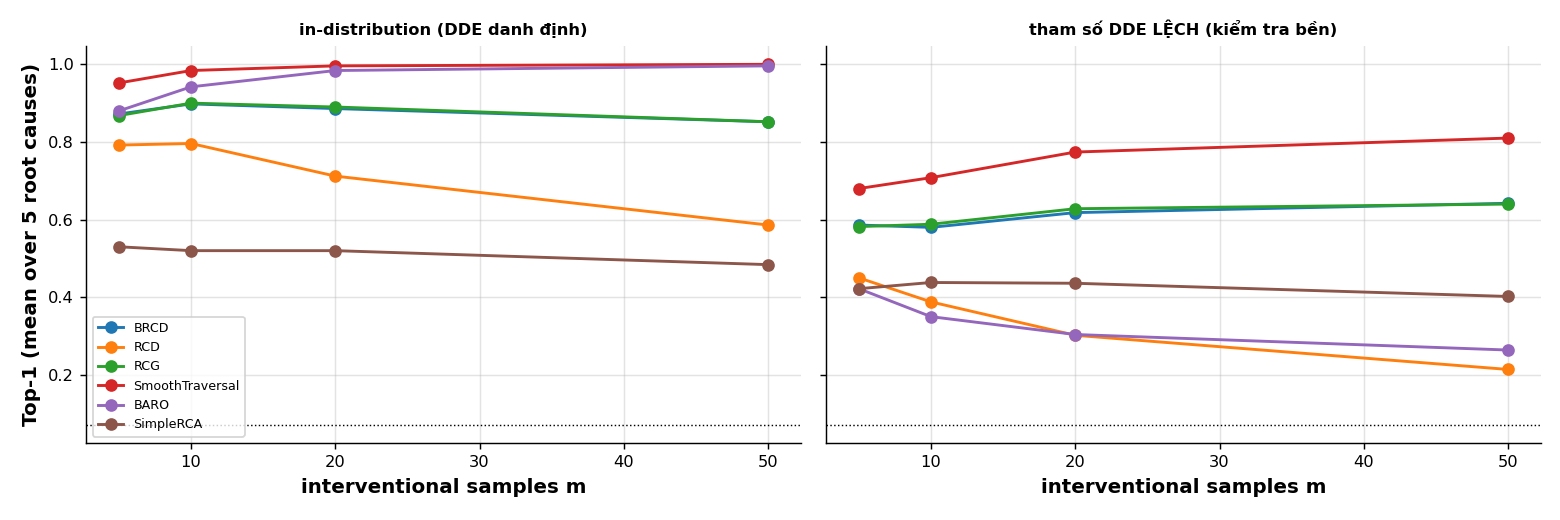
\includegraphics[width=0.95\linewidth]{figures/rca_causal.png}
\caption{Top-1 accuracy of the causal algorithms versus $m$ for the shared-generator and shifted settings (dotted line: chance).}\label{fig:causal}
\end{figure}

\subsection{Dependence on the assumed fault strength}
Scaling the fault gains by $0.3$ and $3$ changes the best classifier's accuracy from $0.698$ to $0.943$ (Table~\ref{tab:sweep}).
Since the gain is set by an assumption, any single accuracy figure from this benchmark should be read together with this curve.
\begin{table}[t]\centering\small
\begin{tabular}{lccc}
\toprule
Classifier & gain $\times 0.3$ & $\times 1$ (calibrated) & $\times 3$ \\
\midrule
Gradient boosting & 0.698 & 0.882 & 0.943 \\
Random forest & 0.674 & 0.855 & 0.922 \\
QDA (Bayes) & 0.545 & 0.769 & 0.847 \\
Logistic regression & 0.535 & 0.729 & 0.834 \\
\bottomrule
\end{tabular}

\caption{Top-1 accuracy of classifiers on simulated data versus fault gain relative to the calibrated value.}\label{tab:sweep}
\end{table}

\subsection{What drives the accuracy? Ablations}\label{sec:ablation}
Table~\ref{tab:ablation} reports $m{=}10$ top-1 accuracy averaged over five root causes, with mean $\pm$ standard deviation over three seeds (each seed changes the cut split and the generated data; 60 draws per fault).
Three observations follow.
First, replacing the physical causal graph by a graph with random edges of the same out-degrees, or by an empty graph, changes no algorithm's accuracy beyond the seed spread (for example BRCD $0.92\pm0.01$, $0.92\pm0.02$ and $0.92\pm0.00$ in the shared-generator setting, and $0.60\pm0.05$, $0.60\pm0.05$ and $0.58\pm0.06$ when shifted).
Because every root-cause node is a graph root, the conditional models of the causal methods cannot add information about those nodes, and the methods act as marginal shift detectors on the node estimates.
Second, replacing the supervised soft sensors by label-free spectral summaries (spectral centroid and peakiness of the 1--3.2~kHz band, low and high microphone bands) reduces accuracy to $0.07$--$0.29$ (shared generator) and $0.07$--$0.37$ (shifted), against a chance level of $0.07$; the simplest method reaches exactly $0.20$, consistent with only the controller-measured spindle-speed node remaining informative (one of five causes), which we did not test directly.
Third, under shifted simulator parameters a larger fault gain does not help: accuracy falls from $0.60$ to $0.27$ for BRCD and from $0.71$ to $0.28$ for Smooth Traversal when the gain is multiplied by 3, because the soft sensors, trained on nominal parameters, mis-estimate the larger and distorted effects.
\begin{table}[t]\centering\footnotesize
\begin{tabular}{p{5.6cm}cccccc}
\toprule
Variant & BRCD & RCD & RCG & Smooth & BARO & Simple \\
\midrule
\multicolumn{7}{l}{\textit{Same generator}} \\
Supervised nodes, physics graph, gain $\times1$ (main setting) & 0.92$\pm$0.01 & 0.81$\pm$0.03 & 0.92$\pm$0.01 & 0.99$\pm$0.00 & 0.91$\pm$0.07 & 0.54$\pm$0.00 \\
Supervised nodes, \emph{shuffled} graph & 0.92$\pm$0.02 & 0.81$\pm$0.03 & 0.92$\pm$0.01 & 0.99$\pm$0.00 & 0.91$\pm$0.07 & 0.54$\pm$0.00 \\
Supervised nodes, \emph{no edges} & 0.92$\pm$0.00 & 0.81$\pm$0.02 & 0.92$\pm$0.00 & 0.99$\pm$0.00 & 0.91$\pm$0.07 & 0.54$\pm$0.00 \\
\emph{Label-free} nodes, physics graph & 0.09$\pm$0.01 & 0.10$\pm$0.04 & 0.07$\pm$0.01 & 0.29$\pm$0.08 & 0.29$\pm$0.08 & 0.20$\pm$0.00 \\
Supervised nodes, physics graph, gain $\times0.3$ & 0.85$\pm$0.02 & 0.78$\pm$0.04 & 0.85$\pm$0.02 & 0.88$\pm$0.05 & 0.65$\pm$0.18 & 0.51$\pm$0.01 \\
Supervised nodes, physics graph, gain $\times3$ & 0.85$\pm$0.02 & 0.76$\pm$0.05 & 0.84$\pm$0.02 & 0.99$\pm$0.01 & 0.97$\pm$0.01 & 0.53$\pm$0.04 \\
\midrule
\multicolumn{7}{l}{\textit{Shifted DDE parameters}} \\
Supervised nodes, physics graph, gain $\times1$ (main setting) & 0.60$\pm$0.05 & 0.43$\pm$0.05 & 0.60$\pm$0.07 & 0.71$\pm$0.07 & 0.39$\pm$0.05 & 0.45$\pm$0.01 \\
Supervised nodes, \emph{shuffled} graph & 0.60$\pm$0.05 & 0.42$\pm$0.05 & 0.59$\pm$0.06 & 0.71$\pm$0.07 & 0.40$\pm$0.05 & 0.45$\pm$0.01 \\
Supervised nodes, \emph{no edges} & 0.58$\pm$0.06 & 0.42$\pm$0.05 & 0.58$\pm$0.06 & 0.70$\pm$0.06 & 0.39$\pm$0.06 & 0.45$\pm$0.01 \\
\emph{Label-free} nodes, physics graph & 0.09$\pm$0.01 & 0.14$\pm$0.04 & 0.07$\pm$0.01 & 0.27$\pm$0.03 & 0.37$\pm$0.02 & 0.20$\pm$0.00 \\
Supervised nodes, physics graph, gain $\times0.3$ & 0.54$\pm$0.03 & 0.45$\pm$0.05 & 0.53$\pm$0.03 & 0.59$\pm$0.03 & 0.48$\pm$0.02 & 0.42$\pm$0.02 \\
Supervised nodes, physics graph, gain $\times3$ & 0.27$\pm$0.07 & 0.22$\pm$0.01 & 0.26$\pm$0.07 & 0.28$\pm$0.09 & 0.22$\pm$0.01 & 0.32$\pm$0.07 \\
\bottomrule
\end{tabular}

\caption{Ablation of the causal RCA benchmark at $m{=}10$: top-1 accuracy (mean $\pm$ s.d.\ over 3 seeds) for the node construction, the graph and the fault gain; chance $=0.07$.}\label{tab:ablation}
\end{table}

\subsection{Comparison with a real defective tool}\label{sec:real}
Cuts with a documented root cause exist in MSM, but for tools other than the one simulated.
We compare the intentionally defective end mill D$^*$ (12 cuts, 36 windows; dataset 3) with the healthy tool of the same type (64 cuts, 192 windows; dataset 14), both 12.7~mm four-flute on AISI~4140.
The cutting conditions of the two sets do not coincide, so we fit a ridge model of each sensor node on the conditions using the healthy cuts only (out-of-sample over cuts), express the defective windows as residuals in units of the healthy residual standard deviation, and bootstrap the cuts for 95\% intervals.
We compare this shift vector with the shift vector of each simulated fault (Table~\ref{tab:realshift}).
The real defective tool raises all node levels, with the largest shifts at low frequency ($+3.9$ and $+4.0$ standard deviations for the 50--600~Hz bands of the accelerometer and the microphone) and in the 1--3.2~kHz accelerometer band ($+6.3$), and lowers both non-synchronous indices ($-3.7$ and $-1.2$), i.e.\ the spectrum becomes more tonal.
No simulated fault produces a low-frequency shift (all within $\pm0.1$) or a comparable change of the non-synchronous indices ($-0.3$ to $+0.5$); the simulated shifts consist of increases of broadband and high-frequency levels.
The cosine similarity between the real and the simulated shift vectors is $0.55$--$0.62$ for all five causes; tool wear is the most similar in 89\% of bootstrap resamples, but the absolute differences between causes are small, since the similarity is dominated by the common ``louder'' direction.
We therefore cannot claim that the simulator reproduces the signature of a defective tool, and the missing low-frequency and tonal components point to a mechanism absent from our fault models (we did not model flute chipping, which creates a strong once-per-revolution component; this is a hypothesis we have not tested).
The two tools differ (12.7~mm, four flutes, steel versus the simulated 6.35~mm, two flutes, aluminium), so this comparison tests only the direction and sign of the shifts in standardised units.
\begin{table}[t]\centering\footnotesize
\begin{tabular}{lcccccc}
\toprule
 & Real defective tool & Stiff. & Damp. & Wear & Depth & RPM \\
\midrule
log acc.\ rms & +1.9 [+1.4, +2.5] & +2.9 & +2.9 & +1.9 & +2.9 & +3.0 \\
mic.\ level & +3.6 [+3.2, +4.1] & +2.3 & +2.4 & +1.4 & +2.3 & +2.4 \\
non-sync.\ (acc) & -3.7 [-4.3, -3.1] & -0.0 & -0.3 & -0.3 & -0.2 & +0.3 \\
non-sync.\ (mic) & -1.2 [-1.5, -0.9] & +0.1 & -0.2 & -0.2 & -0.2 & +0.5 \\
acc.\ 50--600\,Hz & +3.9 [+3.5, +4.2] & -0.0 & +0.0 & -0.0 & -0.0 & +0.0 \\
acc.\ 1--3.2\,kHz & +6.3 [+5.6, +7.1] & +1.8 & +1.2 & +1.0 & +1.3 & +1.5 \\
acc.\ $>$3.2\,kHz & +1.9 [+1.4, +2.3] & +1.5 & +1.3 & +1.5 & +2.1 & +2.1 \\
mic.\ 50--600\,Hz & +4.0 [+3.3, +4.7] & -0.0 & +0.0 & +0.0 & -0.0 & +0.1 \\
mic.\ $>$3.2\,kHz & +1.8 [+1.2, +2.3] & +0.2 & +0.2 & +0.1 & +0.3 & +0.3 \\
\midrule
cosine with real shift & -- & 0.62 & 0.60 & 0.62 & 0.59 & 0.55 \\
\bottomrule
\end{tabular}

\caption{Shift of each sensor node in units of the healthy standard deviation: real defective tool D$^*$ (with 95\% bootstrap intervals over cuts) versus the five simulated faults.}\label{tab:realshift}
\end{table}

\section{Limitations and What Remains}\label{sec:limits}
\begin{itemize}
\item \textbf{No validation of the RCA ranking on real root causes.} The only real comparison (Section~\ref{sec:real}) concerns the signature of one cause on a tool different from the simulated one, and the simulator fails to reproduce its largest components. Clamp-failure and depth cases are single cuts on other tools and were not analysed.
\item \textbf{The benchmark does not test causal reasoning.} Graph ablations show no effect (Section~\ref{sec:ablation}), and node construction decides the result; a benchmark in which root causes are not graph roots with supervised estimates, or in which the graph carries information, would be needed to compare causal algorithms.
\item \textbf{Baseline realism.} The healthy baseline is distinguishable from real data (balanced accuracy 0.78--0.90 across variants and splits) and we could not measure a floor.
\item \textbf{Assumed quantities.} Fault severity ranges, gains, nominal physical parameters and the causal graph are assumptions; force coefficients and tool-tip dynamics for this tool had no verified source.
\item \textbf{Scope.} One tool, one workpiece material, one machine, 73 cuts, mostly up- versus down-milling as the real abnormal signal.
\item \textbf{Seeds.} The main causal and classification tables use one cut split and one generation seed; only the ablation (Table~\ref{tab:ablation}) reports spread over three seeds, and the soft-sensor training uses supervision from the simulator.
\item \textbf{Open hypothesis.} We suspect that the 1.5--2.3~kHz cluster is a tool-structure mode excited when a harmonic of the tooth-passing frequency is close to it; adding a harmonic-proximity feature did not give a clear improvement.
\end{itemize}

\section{Conclusion}
A simulator grounded in real healthy spectra lets us run causal RCA algorithms on machining faults with known causes, but the resulting accuracy depends on how much the diagnostic nodes share with the generator, and falls from near 1.0 to 0.35--0.71 under moderate mismatch of the simulator's physical parameters.
Ablations show that the causal graph plays no role in this benchmark, that label-free node estimates give near-chance accuracy, and that the simulator does not reproduce the low-frequency and tonal signature of a real defective tool.
This is a measurement of the dependence of a simulated benchmark on its assumptions and on node construction, not a claim about real machining diagnosis.

\paragraph{Code and data.}
Code: \texttt{cutting\_sim/} in the project repository (branch \texttt{cutting-sim-experiments}); data: MSM \citep{kim2026msm} (CC BY 4.0). \todo{release instructions}

\bibliographystyle{plainnat}
\bibliography{refs}

\appendix
\section{Parameter provenance}\label{app:registry}
\begin{table}[h]\centering\small
\begin{tabular}{p{5.2cm}p{1.8cm}p{6.5cm}}
\toprule
Parameter & Tier & Verification \\
\midrule
tool diameter, flutes, flute length, overall length & FIXED & verified (read from catalog table p.5) \\
helix angle $\beta$ & FIXED & medium: from series feature list (p.3); not stated per part number \\
tool substrate/coating & FIXED & medium \\
N, ae, feed F, direction & FIXED & verified (N and F equal mtc Spindle\_Speed/Feed\_Rate, ratio 1.000) \\
axial depth ap = engaged depth & FIXED & assumption (not measured) \\
workpiece AA 6061; wet cutting (coolant flood) & FIXED & verified (stated in paper) \\
sampling: accelerometer 51.2 kHz, audio 48 kHz & FIXED & verified (stated in paper) \\
analysis window 0.3 s & FIXED & design choice \\
model structure: regenerative DDE, shear+edge force, ZOA lobes & FIXED & model structure \\
Kt, Kr, Kte, Kre (AA 6061, this tool, wet) & LEARNED & NO usable source (rejected: steel-like values; dry-cutting AA6061 value unverified) \\
tool-tip FRF: fn\_x, fn\_y, $\zeta$, modal stiffness k & LEARNED & NO source for this tool/holder/stick-out (Altintas Ex.2 FRF rejected: different machine and tool) \\
spindle imbalance U & LEARNED & NO source (rotor mass, balance grade unknown) \\
sensor gains, noise floors, rpm-dependence & LEARNED & NO source (sensors uncalibrated: mic dBFS, accelerometer mm/s\^{}2) \\
runout; between-cut variability $\sigma$ (Kt, runout, roughness) & LEARNED & NO source \\
chip-thickness cap 0.3 mm; roughness noise base 0.02 $\mu$m & ASSUMED & own assumption \\
\bottomrule
\end{tabular}

\caption{Every simulator parameter, its tier (fixed / learned / assumed) and verification status.}
\end{table}

\section{Methodological pitfalls found along the way}
\begin{enumerate}
\item Plain accuracy of a classifier two-sample test with unequal sample sizes has a chance level above 0.5; use balanced accuracy.
\item Real and simulated features must be computed on windows of identical length; a 20-fold mismatch changed the apparent variance threefold.
\item Out-of-sample residuals are needed to estimate between-cut variation when the regression can interpolate each cut.
\item Distribution matching alone did not identify the fault gain; effect-size matching was used instead.
\item Nodes of a causal graph that are trained on the generator's labels make the benchmark circular.
\end{enumerate}
\end{document}
